\chapter{Swarmalators on a complete network}

\section{Model presentation}

This model attempts to describe the simultaneous swarming (self-organization of positions in space) and synchronization (self-organization of internal states in time) observed in groups of animals. However, the resulting conclusions may also be applicable to other types of systems, such as colloidal suspensions of magnetic particles \cite{osti_1344461,Snezhko2011MagneticMO,Yan2012LinkingST}. In many frameworks, those two behaviors—swarming and synchronization—interact. For instance some population of myxobacteria appear to have a biochemical degree of freedom (d.o.f.), which can be modeled as a phase. Evidence suggests the presence of a bidirectional coupling between spatial and phase dynamics \cite{igoshin2001pattern}. Another example can be chemotactic oscillators, whose movements in space are mediated by the diffusion of a background chemical \cite{iwasa2010hierarchical,tanaka2007general}.

%For instance, various species of frogs, crickets, and katydids exhibit periodic calling, often synchronizing in large choruses, while moving. \cite{aihara2014spatio,article,greenfield1994synchronous,walker1969acoustic}.

In our treatment we considered a generalization of the Kuramoto model \cite{Acebron_2005} on a network \cite{Rodrigues_2016}, where we ignored alignment (which would have required an additional d.o.f.), and we associated to each node at time t a phase and a position in the xy plane, as in \cite{O_Keeffe_2017, Sar_2022}:

% Position dynamics equation
\begin{equation}
\label{r_swarm}
\frac{d\mathbf{x}_i}{dt} = \mathbf{v}_i + \frac{1}{k_i} \sum_{j=1}^{N} A_{ij}\left[ \frac{\mathbf{x}_j - \mathbf{x}_i}{|\mathbf{x}_j - \mathbf{x}_i|} \left(A + J \cos(\theta_j - \theta_i)\right) - B\frac{\mathbf{x}_j -  \mathbf{x}_i}{|\mathbf{x}_j - \mathbf{x}_i|^2} \right]
\end{equation}

% Phase dynamics equation


\begin{equation}
\label{theta_swarm}
\frac{d\theta_i}{dt} = \omega_i + \frac{K}{k_i} \sum_{j= 1}^{N} A_{ij} \frac{\sin(\theta_j - \theta_i)}{|\mathbf{x}_j - \mathbf{x}_i|}
\end{equation}


\begin{multicols}{2}
\begin{description}[noitemsep]
    \item[\(\mathbf{x}_i\)]: Position vector of the \(i\)th swarmalator in space
    \item[\(\theta_i\)]: Phase of the \(i\)th swarmalator
    \item[\(\mathbf{v}_i\)]: Self-propulsion velocity vector
    \item[\(\omega_i\)]: Natural frequency
    \item[\(A_{ij}\)]: Element of the adjacency matrix of the network
    \item[\(k_i\)]: Degree of node \(i\)
\end{description}
\begin{description}[noitemsep]
    \item[\(N\)]: Total number of swarmalators in the system
    \item[\(J\)]: Position-phase coupling constant
    \item[\(K\)]: Synchronization coupling constant
    \item[\(A\)]: Amplitude of the simple attraction term
    \item[\(B\)]: Amplitude of the repulsion term
\end{description}
\end{multicols}

From now on we set
$$A=B=1 \;\;\;\;\;\; \mathbf{v}_i = \mathbf{0} \;\;\;\;\;\; \omega_i=0 \: \: \forall i$$
\newline
We firstly considered a complete network and, by means of numerical simulations, we reproduced the different states of the system (described in \cite{O_Keeffe_2017, Sar_2022}) as $J$ and $K$ vary. 

\newpage

\section{Numerical simulations}
For our simulation we relied on the R numerical implementation of the Kuramoto model showed in the third laboratory of this course (which used the deSolve package for numerical handling of ODEs).
We extended the model including the equations of motion paying attention not to have singular initial conditions. Luckily \cite{ha2019emergent} ensures that, given initial non-collisional data (initial phases and positions were uniformly generated in $\left[ 0,2 \pi \right[ \times \left[ 0,1 \right]^2$, with the previous presciption), a minimal inter-particle distance among the swarmalators is guaranteed. Even so we still checked the distance matrix at every step to prevent numerical divergence in eq. (\ref{r_swarm})-(\ref{theta_swarm}).
%details of the repulsion function ????

We chose the number of swarmalators $N=300$, step of integration $dt=0.05$ and $T=2000$ timesteps (in fig.\ref{fig:splinter_phase_wave} more steps were necessary to reach the final configuration).
We reproduced the noise-free states illustratated in fig 2 and fig 5 of \cite{O_Keeffe_2017}:

\begin{enumerate}
    \item Static synchrony (fig. \ref{fig:static_sync}): the swarmalators form a cirulary simmetric, crystal-like distribution in space, and are fully synchronized in phase.
    \item Static asynchrony (fig. \ref{fig:static_async}): at any given location $\mathbf{x}$ all phases $\theta$ can occur.
    \item Static phase wave (fig. \ref{fig:static_phase_wave}): since in this special case $K=0$ swarmalators' phases are frozen at their initial values. Still, since $J >0$, units want to settle near others with similar phase.
    \item Splintered phase wave (fig. \ref{fig:splinter_phase_wave}): moving to $K<0$ static phase wave spinters into disconnected clusters of distinct phases where nodes execute small ampltiude oscillations in position and phase.
    \item Active phase wave (fig. \ref{fig:active_phase_wave}): as $K$ decreases oscillations increase in amplitude until swarmalators start to execute regular cycles in both space and phase \footnote{This final state is similar to the double milling states found in biological swarms \cite{Carrillo2009}}.
    
    \end{enumerate}



\newcommand{\imagewidth}{0.55\textwidth} % Define a unique size for all images

\begin{figure}[h]
 \centering
    % First row: Phase diagram
    \begin{minipage}{0.55\textwidth}
        \centering
        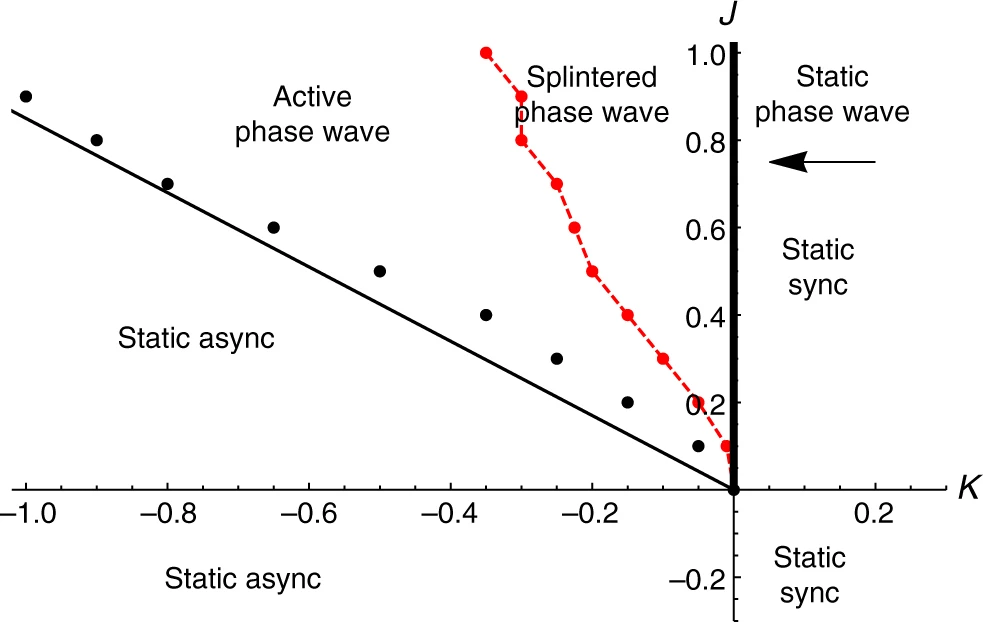
\includegraphics[width=\textwidth]{images/task20/phase_space.png}
        \caption{Phase diagram from \cite{O_Keeffe_2017}.  The straight line separating the static async and active phase wave states is a semi-analytic approximation, while dots are derived from simulation data}
        \label{fig:phase_space}
    \end{minipage}
    \hfill
    % Second row: Static synchronous state and static asynchronous state
    \begin{minipage}{0.4\textwidth}
        \centering
        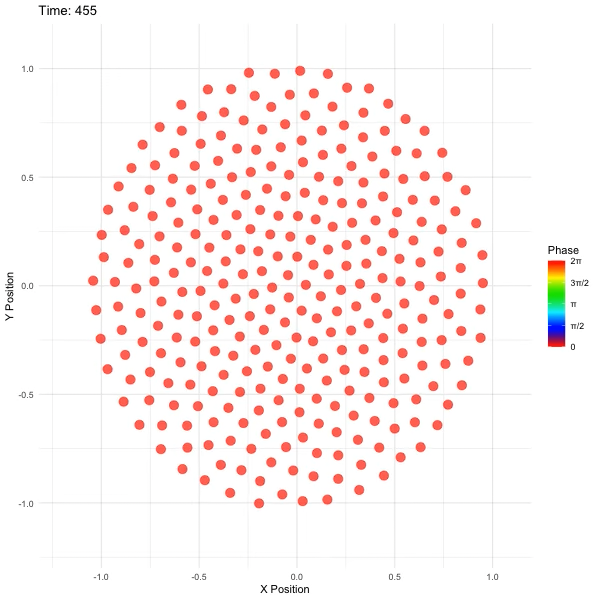
\includegraphics[width=\textwidth]{images/task20/static_sync.png}
        \caption{Static synchronous state \newline ($K=1$, $J=0.1$)}
        \label{fig:static_sync}
    \end{minipage}
\end{figure}






\begin{figure}[p] % Full-page figure

    % Second row: Two smaller images side by side
    \begin{minipage}{\imagewidth}
        \centering
        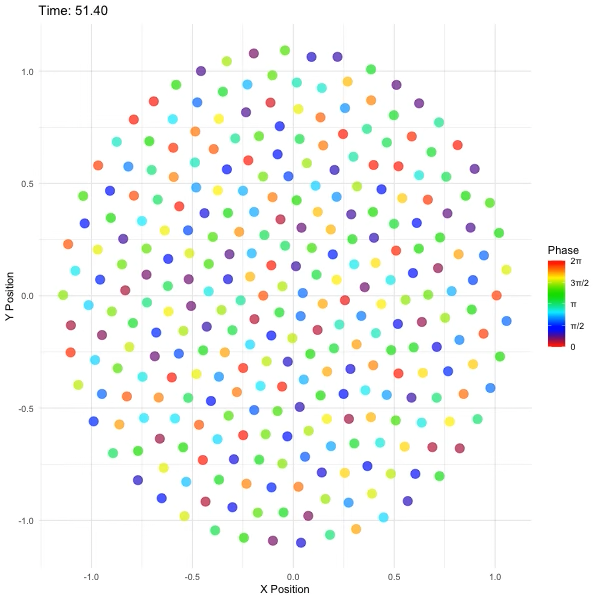
\includegraphics[width=\textwidth]{images/task20/static_async.png}
        \caption{Static asynchronous state \newline ($K=-1$, $J=0.1$)}
        \label{fig:static_async}
    \end{minipage}
    \hfill
    \begin{minipage}{\imagewidth}
        \centering
  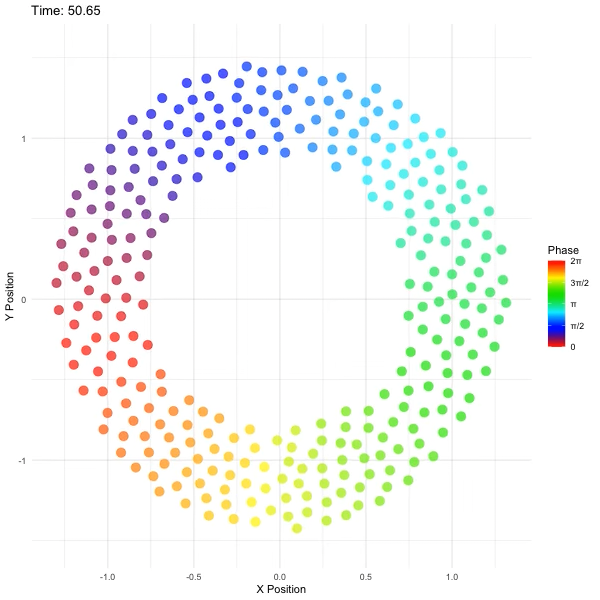
\includegraphics[width=\textwidth]{images/task20/static_phase_wave.png}
    \caption{Static phase wave state\\ \parbox[t]{\textwidth}{\raggedright ($K=0$, $J=1$)}}
    \label{fig:static_phase_wave}
    \end{minipage}

    \vspace{0.8cm} % Space between rows

    % Third row: Two smaller images side by side
    \begin{minipage}{\imagewidth}
        \centering
        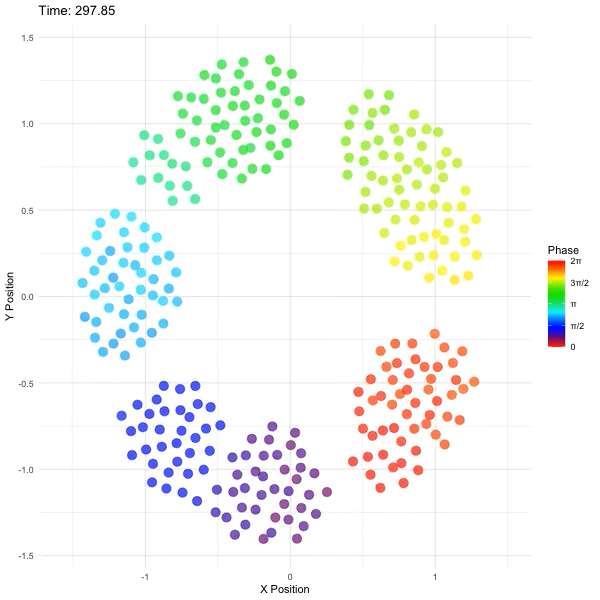
\includegraphics[width=\textwidth]{images/task20/splintered_phase_wave.png}
        \caption{Splinter phase wave  state\newline
        ($K=-0.1$, $J=1$)}
        \label{fig:splinter_phase_wave}
    \end{minipage}
    \hfill
    \begin{minipage}{\imagewidth}
    \centering
    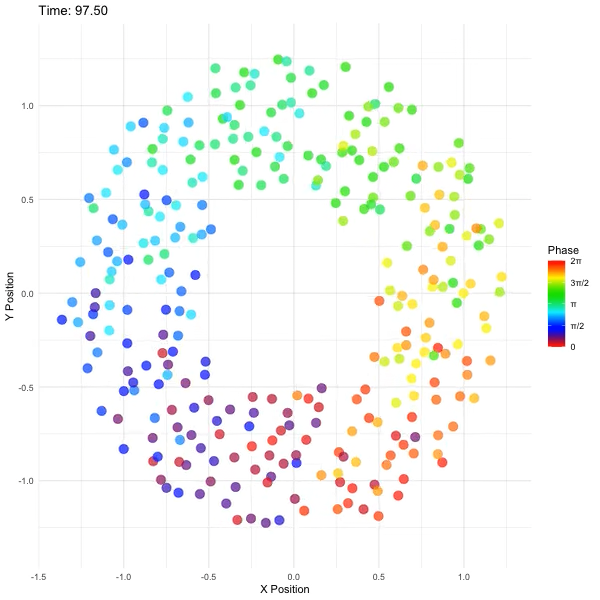
\includegraphics[width=\textwidth]{images/task20/active_phase_wave.png}
    \caption{Active phase wave state \\ \parbox[t]{\textwidth}{\raggedright ($K=-0.6$, $J=0.9$)}}
    \label{fig:active_phase_wave}
\end{minipage}


%    \caption{Various Swarmalator Simulation States}
\end{figure}




